%% Introduction 
%%	What is this chapter all about? 
%%	What sub-problem or issue is this chapter addressing? 
%%	How does this chapter fit within the overall “story” of the thesis? 
%%The Meat
%%	Rigorous approach to sub-problem, or detailed explanation of issue
%%	Assumptions underlying sub-problem, or complete description of issue
%%	Validation: System design, theory, implementation, graphs, references, …. 
%%Summary
%%	Repeat the highlights of the chapter
%%	Transition sentence that acts as a “teaser” for the next chapter, and how the next chapter fits with the current one

\todo{Review comment: Not able to see logical sequence of sections.[WILL TAKE SUGGESTIONS]}

\section{Introduction}

This chapter presents an\deleted{newly proposed} approach for validating the midsurface generated from a CAD model. %Midsurface generated by the proposed approach which has been mentioned in the previous chapters, is tested for correctness and errors, if any.

\todo{Review comment: Mention that midsurface are generated by your algorithm in chapter 6. [DONE]}

Midsurface, as defined by Rezayat~\cite{Rezayat1996}, is expressed as a contiguous flow of the input solid (Definition~\ref{def:midsrez}). Midsurface is expected to lie midway and be representative of the input solid. The first part of the requirement, i.e. `lying midway' is geometrical in nature whereas being `representative' is topological in nature. Geometrical validation approaches check if the midsurface is at half the distance from side-faces of the input solid. Topological validation approaches check if the midsurface has similar connectivities between its sub-shapes as in the input solid. These validations help detect errors in midsufaces, such as missing midsurface patches, gaps or overlaps amongst them, midsurface not lying midway, etc.


%%\bigskip

\begin{figure}[!h]
\centering     %%% not \center
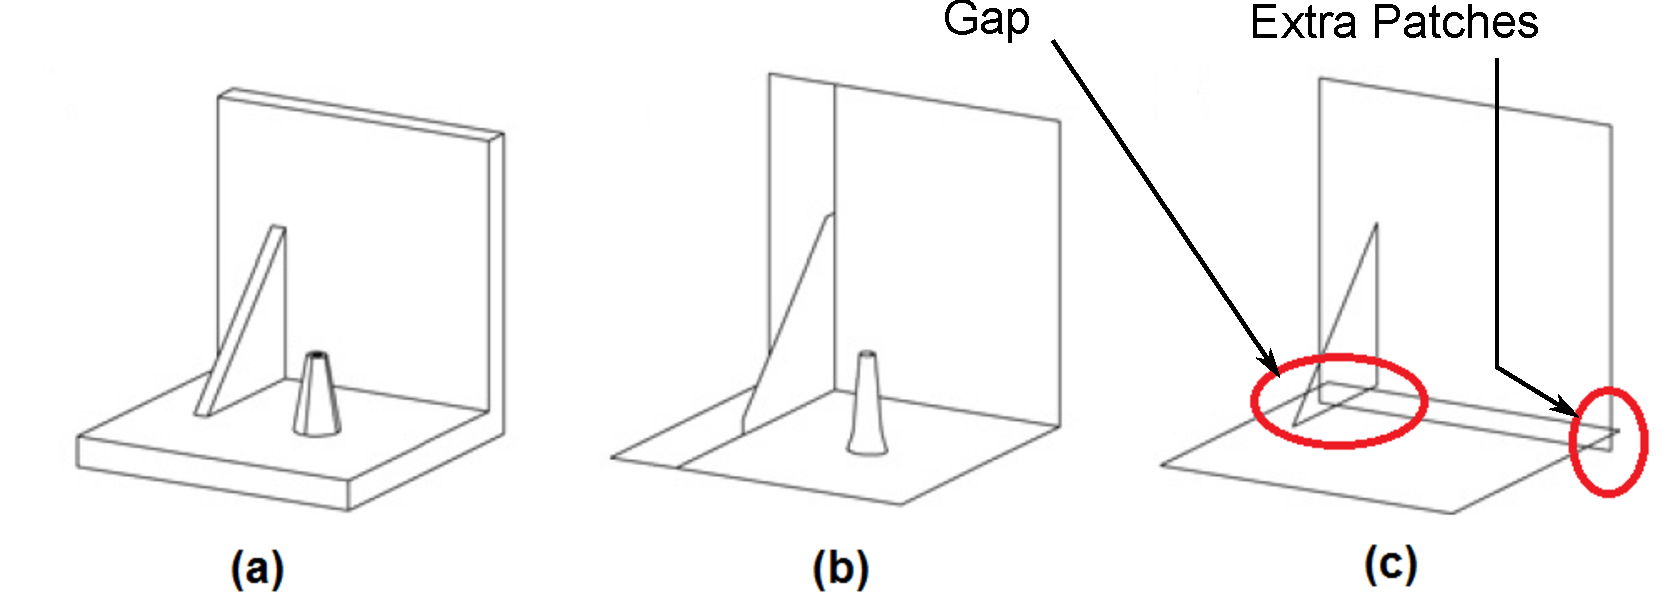
\includegraphics[width=0.8\linewidth,valign=t]{images/midslocketterrors.pdf}
\caption{Model, Good Midsurface, Bad Midsurface (Source: Lockett~\cite{Lockett2008}}
\label{fig:litsurvey:midslocketterrors}
\end{figure}

%%\bigskip

Figure~\ref{fig:litsurvey:midslocketterrors}(a) shows an example input model. Figure~\ref{fig:litsurvey:midslocketterrors}(b) shows a correct output, i.e. a well connected midsurface. Figure~\ref{fig:litsurvey:midslocketterrors}(c) shows midsurface output with errors such as gaps and extra patches. Various approaches are used to detect such errors.

Traditionally, midsurface validations are done using following methods or tools:

\begin{itemize}
[noitemsep,topsep=2pt,parsep=2pt,partopsep=2pt]
\item \textbf{Manual}: Manual inspection is done to ensure that the midsurface lies midway and is continuous throughout, especially at the junctions. If any errors are found, such as gaps or overlaps, they are corrected manually by using available modeling operations such as extend or trim.  This technique is obviously tedious, time-consuming and error-prone, because detecting errors and correcting them in complex parts is difficult.
\item \textbf{Semi-automatic Tools}: Ready tools are provided by CAD-CAE systems which can detect gaps and overlaps, automatically. In some cases functionalities such as ``auto-heal'' or ``auto-fill'' are provided to put surface patches at the site of gaps or holes in the midsurface. These tools have limited applicability as the automatic detection and healing is not robust and does not work consistently for complex geometries. Also, these tools cannot detect correctness topologically, i.e. appropriateness of the connections of midsurface patches.
\item \textbf{Automatic Distance Comparison}: Automatic tools are provided to check if distance between midsurfaces and the input solid is half the thickness. Hausdorff distance~\cite{Lockett2008}, which measures maximum dissimilarity between two shapes, is used for assessing geometric similarity. But, as pointed by Lockett ~\cite{Lockett2008}, this technique does not work in some valid situations, such as at junctions, where the distances can be more than half the thickness.%%\item \textbf{Topological Validation}: This involves use of topological entities for comparison with the ideal output. Here, the geometry of the shape, is ignored. It has an advantage over geometric validation since computationally intensive distance calculations are not performed. 
\end{itemize}

All the above mentioned tools are used mainly for geometric validations. Following section evaluates some of the traditional validation approaches and establishes need for a new topological validation approach.

\section{Need for Topological Validation}\label{sec:topoval:need}

Review of the traditional techniques suggests that the `Manual' and the `Semi-automatic' techniques are cumbersome to use, especially in cases of large and complex midsurfaces. The automatic validation technique of distance comparison is thus a preferred method for complex midsurfaces. In this technique, Hausdorff distance between corresponding faces on the input solid are measured and checked if they are half of the given thickness. 

Eqn~\ref{eqn:Hausdorff} defines Hausdorff distance between two surfaces.% as the maximum over all the points in A of the minimum distances to B. 
\begin{equation*}\label{eqn:Hausdorff}  
\begin{aligned}
\bar{h}(A,B) = max_{a \in A} min_{b \in B} d(a,b) \\
H(A,B) = max (\bar{h}(A,B),\bar{h}(B,A))
\end{aligned}
\end{equation*}

$\bar{h}(A,B)$ gives maximum value amongst the least values of distances from sample points ($a$) on surface $A$ to sample points ($b$) on surface $B$. The process is repeated in the other direction i.e. $\bar{h}(B,A)$. The maximum between these two values is the Hausdorff distance.

Figure~\ref{fig:litsurvey:housdorff} shows a sample computation of distance between $a$ and $b$ points on surface $A$ and $B$ respectively. Minimum of these distances is computed first. Then maximum from all sample $a$ points is considered as directed Hausdorff distance from $A$ to $B$. Similarly directed Hausdorff distance from $B$ to $A$ is computed. Maximum between these two is considered as the Hausdorff distance. Thus it is a single representative value of distance between two surfaces.

%%\bigskip

\begin{figure}[!h]
\centering     %%% not \center
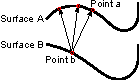
\includegraphics[width=0.35\linewidth,valign=t]{images/hausdorff.pdf}
\caption{Hausdorff Distance between two surfaces}
\label{fig:litsurvey:housdorff}
\end{figure}

%%\bigskip

This technique of checking geometric similarity using Hausdorff distance is widely used in applications such as shape matching, validations, etc. But it has few drawbacks too. The accuracy of the method depends on the number of sample points. More the points better the accuracy but then, more are the distance computations. Apart from this, it does not particularly work at the junctions as the correct distance there can be more than the half of thickness. 

%%\bigskip

\begin{figure}[!h]
\centering     %%% not \center
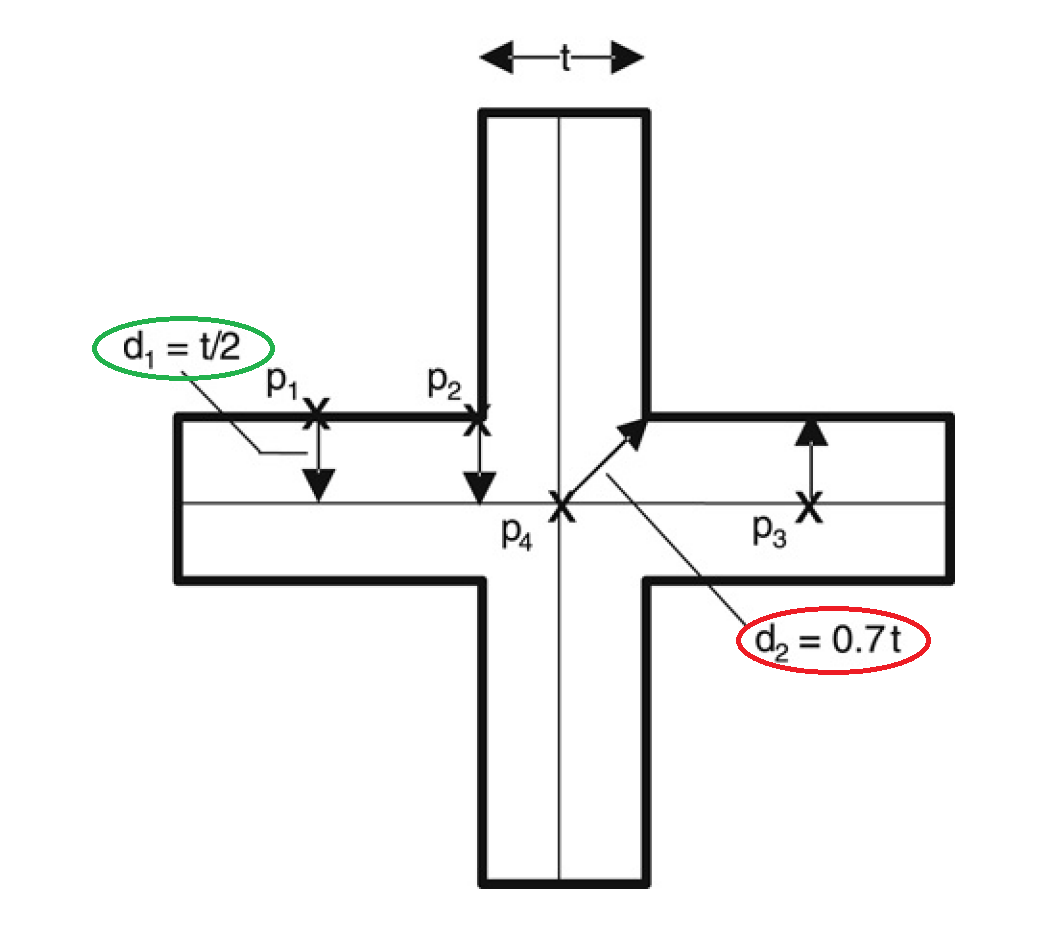
\includegraphics[width=0.45\linewidth,valign=t]{images/lockettx}
\caption{Distance at the junction (Source: Lockett~\cite{Lockett2008})}
\label{fig:litsurvey:lockettx}
\end{figure}

%%\bigskip

Figure~\ref{fig:litsurvey:lockettx} shows that distance from points like $p_1$ and $p_2$ to midsurface is $d_1 = t/2$, where $t$ is the thickness. But at the junctions, the distance from midsurface (point $p_4$) to its closest face on the input solid is $0.7t$. Although it is more than the permissible distance of $0.5t$, it is valid. Thus, it is not possible to ascertain the correct threshold for determining validation and so, for geometric validation techniques it is challenging to detect if the distance measured is appropriate or an error.

\todo{Review comment: You have to introduce your work here, also make it clear that it provides a theoretical approach for validating midsurface, however this works has not been implemented in the software system. [DONE]}

Geometric validation technique cannot find missing connections, similarity with the input solid, etc. Thus, to have more complete validation, geometric techniques need to be complemented by topological criteria as well. The present research proposes topological validation method in which topological entities of midsurface are predicted from the input solid's topological entities. Validation is done by comparing the predicted entities with the actual entities of the midsurface. This technique helps find missing gaps, connections, etc. However, being topological, it does not carry out the essential geometric distance calculations, which the existing  geometric validation technique can perform. The approach proposed here for topological validation complements geometric validation and thus makes overall validation of the midsurface more robust.

Following sections present the topological validation approach developed in this research work. It is however noted that this approach is limited to only providing a theoretical framework and is not iimplemented in the software system,~\mysystemname.%The development is only theoretical in nature. Implementation of this approach is, however, left as the future scope. 

To understand the state of the art, relevant works in the domain of topological validation are reviewed in the next section.

%%Even after extensive research in the academic domain and wide availability in commercial implementations, midsurface quality is still a concern. It suffers from errors like gaps, overlaps, missing surfaces, etc. Validating the output midsurface is a critical step in assessing the quality, after which corrective actions can be taken. 
%%The validation method presented in this work cannot be used in isolation from geometry. As the midsurface is applicable only for the thin-walled solids, it is not computed and validated using this method for thick solids. But such differentiation of the solid-shape, being thick or thin, is 'geometrical' and not 'topological', which this method itself cannot detect. So, the work presented below should be used only for the known thin-walled solids for which midsurface are computable. Use of topology for assessing the quality of midsurface is not widespread and there are very few such attempts reported in the literature (Section \ref{sec:litsurvey:validation}). 

%%Many sheet metal CAD modelers represent the thin-walled shape using a data-structure called a Boundary Representation (Brep). Section \ref{sec:topoval:preliminaries}  provides the characteristics of Brep and its classification into manifold and non-manifold representations. In this work, the term 'manifold' refers to an object which is bound, closed and homeomorphic to a topological sphere (also known as 2-manifold), whereas 'non-manifold' object does not have such restrictions of closure and completeness. This work uses 'non-manifold' mainly for surfaces, unless stated otherwise.
%%
%%Following are the ways in which some of the midsurface errors can be detected using the predicted entities:
%%\begin{itemize}
%%[noitemsep,topsep=2pt,parsep=2pt,partopsep=2pt]
%%\item \textbf{Missing Surfaces}: Missing surfaces result in lesser number of edges and vertices
%%\item \textbf{Missing Connections}: Gaps result in lesser radial edges and vertices 
%%\end{itemize}


\section{Related Work}

In past, shape matching applications were being used to find similar parts from CAD databases. Criteria used for checking shape similarity can be classified as geometric and topological. Shape signatures, histograms are geometric, whereas graph based, feature recognition techniques are topological in nature~\cite{Lockett2008}.
%
%Apart from CAE, skeletal structures such as midsurface are used in CAD model comparison solutions such as shape-based retrieval, similarity assessment and difference identification  \cite{Antoine2014}. Skeletal graph matching is one of the prominent techniques \cite{Iyer2005} for similarity assessment. A topologically valid midsurface represents sub-shape connectivities better and thus acts as more effective shape-signature in the model comparison.

In CAD, surfaces are represented by non-manifold topological equations. Lipson~\cite{Lipson} derived equations related to topological invariant for the sheet metal non-manifold model which can be used for topological representation of the midsurface.

Lee~\cite{SHLee2001} presented reverse of midsurface generation approach, called `sheet thickening'. In this approach, a sheet (which can be considered as a midsurface) was offsetted, thickened to form thin-walled model. This work lacked detailed transformation equations.

One of the most significant contribution in the shape similarity assessment, in the context of midsurface, is by Helen Lockett~\cite{Lockett2008}. She developed a methodology to predict topological entities of midsurface by using proximity groups adjusted by angle criterion.

%%\bigskip

\begin{figure}[!h]
\centering     %%% not \center
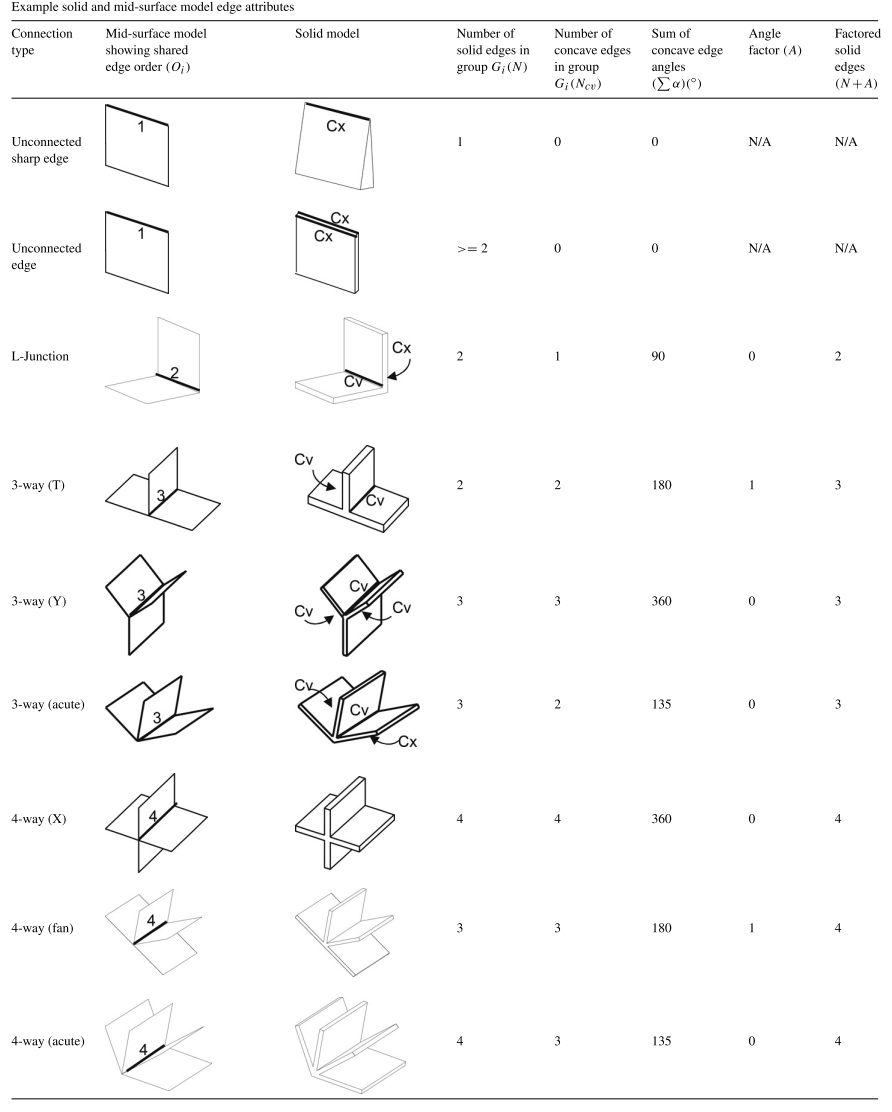
\includegraphics[width=\linewidth,valign=t]{images/locketttopoval}
\caption{Topological Similarity Validation (Source: Lockett~\cite{Lockett2008})}
\label{fig:litsurvey:locketttopoval}
\end{figure}

%%\bigskip

Figure~\ref{fig:litsurvey:locketttopoval} shows Lockett's topological similarity validation technique. For example, in case of ``L'', at junction, the solid model has 2 edges, one concave ($Cv$) and one convex ($Cx$). Out of which, the number of $Cv$ edges is 1. Angle at $Cv$ is $90$, so the predicted faces joining at the junction in the midsurface are 2. 

In case of ``T'', as the sum of angles is $180$, one more edge is added, making the number of edges at the junction as 3. But in case of, ``Y'', which is topologically similar to ``T'', as the sum of angles is $360$, no additional edge is used, making the number of edges at the junction as 3. Thus use of hard-coded rules based on geometric angle values, makes this approach heuristic.

Lockett's topological similarity validation technique shows use of geometric quantities angles, proximity groups, etc. which appears inappropriate. Apart from this, the technique appears limited to only simple academic cases. 
%The present research proposes similar but more generic methodology using puring topological entity equations.


%The present research has derived similar topological invariant with respect to midsurface, to check its correctness.

%% WRITE ALL entries from table here

Table \ref{tbl:survey:topoval} outlines the summary of past research contributions in the relevant topological invariants and similarity assessment approaches:
 
%%\bigskip


\csvreader[longtable=|p{0.12\linewidth}|p{0.12\linewidth}|p{0.15\linewidth}|p{0.2\linewidth}|p{0.15\linewidth}|p{0.15\linewidth}|,
    table head={\toprule \bfseries Author & \bfseries Input& \bfseries  Method& \bfseries  Approach& \bfseries  Advantages& \bfseries  Limitations \\ \midrule \endhead \caption{Survey of Topology Invariants and Validation Approaches}\label{tbl:survey:topoval} \endlastfoot},% \bottomrule \endfoot,
  late after last line=\\\bottomrule,
  before reading={\catcode`\#=12},after reading={\catcode`\#=6},    
    late after line=\\\hline]%
    		{litsurvey_validation.csv}
    		{Author=\Author, Input=\Input, Method=\Method, Approach=\Approach, Advantages=\Advantages ,Limitations=\Limitations}%
    		{\Author  & \Input&  \Method &\Approach & \Advantages & \Limitations}%

%%\bigskip


Review of the reported works has observed that, topological validation approaches are not prevalent. The ones which use topological criteria appear to be using some geometric criteria as well, making them susceptible to geometric errors. Thus, there is need to devise a fully topology based validation technique, specifically for assessing the output midsurface.

Following sections present the proposed approach for topologically validating the output midsurface.

%%% NO CITATIONS IN OBSREVATOINS

%\subsection{Observations on Midsurface Validation Approaches}
%
%\begin{itemize}[noitemsep,topsep=2pt,parsep=2pt,partopsep=2pt]
%\item Apart from CAE, skeletal structures such as midsurface are used in CAD model comparison solutions such as shape-based retrieval, similarity assessment and difference identification  \cite{Antoine2014}. 
%\item Skeletal graph matching is one of the prominent approaches \cite{Iyer2005} for similarity assessment. 
%\item A topologically valid midsurface represents sub-shape connectivities better and thus acts as more effective shape-signature in the model comparison.
%
%\end{itemize}

%%
%%\section{The Need for Topological Validation}
%%
%%%%Even after extensive research in the academic domain and wide availability in commercial implementations, midsurface quality is still a concern. It suffers from errors like gaps, overlaps, missing surfaces, etc. Validating the output midsurface is a critical step in assessing the quality, after which corrective actions can be taken. 
%%%%The validation method presented in this work cannot be used in isolation from geometry. As the midsurface is applicable only for the thin-walled solids, it is not computed and validated using this method for thick solids. But such differentiation of the solid-shape, being thick or thin, is 'geometrical' and not 'topological', which this method itself cannot detect. So, the work presented below should be used only for the known thin-walled solids for which midsurface are computable. Use of topology for assessing the quality of midsurface is not widespread and there are very few such attempts reported in the literature (Section \ref{sec:litsurvey:validation}). 
%%
%%Many sheet metal CAD modelers represent the thin-walled shape using a data-structure called a Boundary Representation (Brep). Section \ref{sec:topoval:preliminaries}  provides the characteristics of Brep and its classification into manifold and non-manifold representations. In this work, the term 'manifold' refers to an object which is bound, closed and homeomorphic to a topological sphere (also known as 2-manifold), whereas 'non-manifold' object does not have such restrictions of closure and completeness. This work uses 'non-manifold' mainly for surfaces, unless stated otherwise.
%%
%%Following are the ways in which some of the midsurface errors can be detected using the predicted entities:
%%\begin{itemize}
%%[noitemsep,topsep=2pt,parsep=2pt,partopsep=2pt]
%%\item \textbf{Missing Surfaces}: Missing surfaces result in lesser number of edges and vertices
%%\item \textbf{Missing Connections}: Gaps result in lesser radial edges and vertices 
%%\end{itemize}
%%
%%
%%
%%To verify the quality of the midsurface, the following methods are used:
%%
%%\begin{itemize}
%%[noitemsep,topsep=2pt,parsep=2pt,partopsep=2pt]
%%\item \textbf{Manual}: Manual inspection to ensure that the midsurface lies midway and is continuous throughout, especially on the connections and steps. This method is obviously tedious, time-consuming and error-prone.
%%\item \textbf{Inspection Tools}: Tools provided in the CAD-CAE packages can detect gaps and overlaps, but they cannot detect the correctness of the midsurface at critical locations, such as connections and steps, where expectations could be  subjective.
%%\item \textbf{Geometric Tools}: Hausdorff distance from the midsurface to its input shape is computed to verify that it lies midway. The accuracy depends on the sampling as well as on the complexity of the surface representation, making them computationally intensive and error-prone. 
%%\item \textbf{Topological Validation}: This involves use of topological entities for comparison with the ideal output. Here, the geometry of the shape, is ignored. It has an advantage over geometric validation since computationally intensive distance calculations are not performed. 
%%\end{itemize}
